\documentclass{book}
\usepackage[a4paper,top=2.5cm,bottom=2.5cm,left=2.5cm,right=2.5cm]{geometry}
\usepackage{makeidx}
\usepackage{natbib}
\usepackage{graphicx}
\usepackage{multicol}
\usepackage{float}
\usepackage{listings}
\usepackage{color}
\usepackage{ifthen}
\usepackage[table]{xcolor}
\usepackage{textcomp}
\usepackage{alltt}
\usepackage{ifpdf}
\ifpdf
\usepackage[pdftex,
            pagebackref=true,
            colorlinks=true,
            linkcolor=blue,
            unicode
           ]{hyperref}
\else
\usepackage[ps2pdf,
            pagebackref=true,
            colorlinks=true,
            linkcolor=blue,
            unicode
           ]{hyperref}
\usepackage{pspicture}
\fi
\usepackage[utf8]{inputenc}
\usepackage{mathptmx}
\usepackage[scaled=.90]{helvet}
\usepackage{courier}
\usepackage{sectsty}
\usepackage{amssymb}
\usepackage[titles]{tocloft}
\usepackage{doxygen}
\lstset{language=C++,inputencoding=utf8,basicstyle=\footnotesize,breaklines=true,breakatwhitespace=true,tabsize=4,numbers=left }
\makeindex
\setcounter{tocdepth}{3}
\renewcommand{\footrulewidth}{0.4pt}
\renewcommand{\familydefault}{\sfdefault}
\hfuzz=15pt
\setlength{\emergencystretch}{15pt}
\hbadness=750
\tolerance=750
\begin{document}
\hypersetup{pageanchor=false,citecolor=blue}
\begin{titlepage}
\vspace*{7cm}
\begin{center}
{\Large Board\-Game \\[1ex]\large 1.\-0 }\\
\vspace*{1cm}
{\large Generated by Doxygen 1.8.3.1}\\
\vspace*{0.5cm}
{\small Sun May 19 2013 13:34:12}\\
\end{center}
\end{titlepage}
\clearemptydoublepage
\pagenumbering{roman}
\tableofcontents
\clearemptydoublepage
\pagenumbering{arabic}
\hypersetup{pageanchor=true,citecolor=blue}
\chapter{Hierarchical Index}
\section{Class Hierarchy}
This inheritance list is sorted roughly, but not completely, alphabetically\-:\begin{DoxyCompactList}
\item \contentsline{section}{Board}{\pageref{class_board}}{}
\item \contentsline{section}{Game}{\pageref{class_game}}{}
\begin{DoxyCompactList}
\item \contentsline{section}{Breaktrough}{\pageref{class_breaktrough}}{}
\item \contentsline{section}{Test\-Game}{\pageref{class_test_game}}{}
\end{DoxyCompactList}
\item \contentsline{section}{Move\-Dir}{\pageref{struct_move_dir}}{}
\item \contentsline{section}{Piece}{\pageref{class_piece}}{}
\begin{DoxyCompactList}
\item \contentsline{section}{Pawn}{\pageref{class_pawn}}{}
\end{DoxyCompactList}
\item \contentsline{section}{Point}{\pageref{struct_point}}{}
\end{DoxyCompactList}

\chapter{Class Index}
\section{Class List}
Here are the classes, structs, unions and interfaces with brief descriptions\-:\begin{DoxyCompactList}
\item\contentsline{section}{\hyperlink{class_board}{Board} \\*Brief description. Gameboard used by class \hyperlink{class_game}{Game}, contains pieces and size etc for common properties and functions for board games }{\pageref{class_board}}{}
\item\contentsline{section}{\hyperlink{class_breaktrough}{Breaktrough} \\*Brief description. Class \hyperlink{class_breaktrough}{Breaktrough} derived from \hyperlink{class_game}{Game} interface class }{\pageref{class_breaktrough}}{}
\item\contentsline{section}{\hyperlink{class_game}{Game} \\*Brief description. Class \hyperlink{class_game}{Game} use as base interface for 2 player board games }{\pageref{class_game}}{}
\item\contentsline{section}{\hyperlink{struct_move_dir}{Move\-Dir} \\*Brief description. Simple struct that indicats how far a piece can move each turn for each direction }{\pageref{struct_move_dir}}{}
\item\contentsline{section}{\hyperlink{class_pawn}{Pawn} \\*Brief description. \hyperlink{class_pawn}{Pawn} is a derived class from \hyperlink{class_piece}{Piece} and implements its own function get\-Moves }{\pageref{class_pawn}}{}
\item\contentsline{section}{\hyperlink{class_piece}{Piece} \\*Brief description. Class \hyperlink{class_piece}{Piece} is a default piece class that can be derived from. And can have different settings and behavior }{\pageref{class_piece}}{}
\item\contentsline{section}{\hyperlink{struct_played_games}{Played\-Games} \\*Brief description. \hyperlink{struct_played_games}{Played\-Games} is a simple struct to handle moves }{\pageref{struct_played_games}}{}
\item\contentsline{section}{\hyperlink{struct_point}{Point} \\*Brief description. struct \hyperlink{struct_point}{Point} simple struct for cords, implements comparision between \hyperlink{struct_point}{Point} instances and assigning values }{\pageref{struct_point}}{}
\end{DoxyCompactList}

\chapter{Class Documentation}
\hypertarget{class_board}{\section{Board Class Reference}
\label{class_board}\index{Board@{Board}}
}


Brief description. Gameboard used by class \hyperlink{class_game}{Game}, contains pieces and size etc for common properties and functions for board games.  




{\ttfamily \#include $<$Board.\-h$>$}

\subsection*{Public Member Functions}
\begin{DoxyCompactItemize}
\item 
\hypertarget{class_board_a9ee491d4fea680cf69b033374a9fdfcb}{\hyperlink{class_board_a9ee491d4fea680cf69b033374a9fdfcb}{Board} ()}\label{class_board_a9ee491d4fea680cf69b033374a9fdfcb}

\begin{DoxyCompactList}\small\item\em default constructor \end{DoxyCompactList}\item 
\hyperlink{class_board_a2a454606767ae96c22a728f3268b10fc}{Board} (int h, int w)
\begin{DoxyCompactList}\small\item\em constructor sets height and width of board \end{DoxyCompactList}\item 
\hypertarget{class_board_abe6ef93a03902a234b541130dab81366}{\hyperlink{class_board}{Board} \& \hyperlink{class_board_abe6ef93a03902a234b541130dab81366}{operator=} (\hyperlink{class_board}{Board} \&rhs)}\label{class_board_abe6ef93a03902a234b541130dab81366}

\begin{DoxyCompactList}\small\item\em assignment operator \end{DoxyCompactList}\item 
std\-::string \hyperlink{class_board_ab4b499dd0102694b8eb2f67f6717f9d3}{Check\-Owner} (int X, int Y)
\begin{DoxyCompactList}\small\item\em Checks for owner of piece placed on provided cord returns string value for player. \end{DoxyCompactList}\item 
void \hyperlink{class_board_a5bef79c659946f9849a3d163f27e5191}{Revert} (\hyperlink{class_board}{Board} G)
\begin{DoxyCompactList}\small\item\em Reverts moves. \end{DoxyCompactList}\item 
void \hyperlink{class_board_abbfb453ac45df0b5b1ca389c3edc3810}{Set\-Size} (int h, int w)
\begin{DoxyCompactList}\small\item\em Sets size of board. \end{DoxyCompactList}\item 
\hypertarget{class_board_a67905f3b441a8605aeb50d8978415aa0}{int \hyperlink{class_board_a67905f3b441a8605aeb50d8978415aa0}{get\-Width} ()}\label{class_board_a67905f3b441a8605aeb50d8978415aa0}

\begin{DoxyCompactList}\small\item\em Returns width of the board. \end{DoxyCompactList}\item 
\hypertarget{class_board_a14466e56568d523e5f4d0d695ccbcce1}{int \hyperlink{class_board_a14466e56568d523e5f4d0d695ccbcce1}{get\-Height} ()}\label{class_board_a14466e56568d523e5f4d0d695ccbcce1}

\begin{DoxyCompactList}\small\item\em Returns height of the board. \end{DoxyCompactList}\item 
\hypertarget{class_board_a9b90253fcbc77e78916f618c51558cc4}{void \hyperlink{class_board_a9b90253fcbc77e78916f618c51558cc4}{Generate\-Board} ()}\label{class_board_a9b90253fcbc77e78916f618c51558cc4}

\begin{DoxyCompactList}\small\item\em Generates board. \end{DoxyCompactList}\end{DoxyCompactItemize}
\subsection*{Public Attributes}
\begin{DoxyCompactItemize}
\item 
\hypertarget{class_board_ac512a2358f2828b75f86de08c7c5bd57}{std\-::vector$<$ std\-::vector$<$ \hyperlink{class_piece}{Piece} $>$ $>$ \hyperlink{class_board_ac512a2358f2828b75f86de08c7c5bd57}{Game\-Board}}\label{class_board_ac512a2358f2828b75f86de08c7c5bd57}

\begin{DoxyCompactList}\small\item\em Vector of gameboards and states of game. \end{DoxyCompactList}\item 
\hypertarget{class_board_ab8f6c7f649ce262ddcb75458e3e1a984}{int \hyperlink{class_board_ab8f6c7f649ce262ddcb75458e3e1a984}{player1\-\_\-pieces}}\label{class_board_ab8f6c7f649ce262ddcb75458e3e1a984}

\begin{DoxyCompactList}\small\item\em Amount of pieces for player 1. \end{DoxyCompactList}\item 
\hypertarget{class_board_a3c60deb1a6669deafa24c3309e61b948}{int \hyperlink{class_board_a3c60deb1a6669deafa24c3309e61b948}{player2\-\_\-pieces}}\label{class_board_a3c60deb1a6669deafa24c3309e61b948}

\begin{DoxyCompactList}\small\item\em Amount of pieces for player 2. \end{DoxyCompactList}\end{DoxyCompactItemize}


\subsection{Detailed Description}
Brief description. Gameboard used by class \hyperlink{class_game}{Game}, contains pieces and size etc for common properties and functions for board games. 

\subsection{Constructor \& Destructor Documentation}
\hypertarget{class_board_a2a454606767ae96c22a728f3268b10fc}{\index{Board@{Board}!Board@{Board}}
\index{Board@{Board}!Board@{Board}}
\subsubsection[{Board}]{\setlength{\rightskip}{0pt plus 5cm}Board\-::\-Board (
\begin{DoxyParamCaption}
\item[{int}]{h, }
\item[{int}]{w}
\end{DoxyParamCaption}
)}}\label{class_board_a2a454606767ae96c22a728f3268b10fc}


constructor sets height and width of board 


\begin{DoxyParams}{Parameters}
{\em h} & heigt \\
\hline
{\em w} & width \\
\hline
\end{DoxyParams}


\subsection{Member Function Documentation}
\hypertarget{class_board_ab4b499dd0102694b8eb2f67f6717f9d3}{\index{Board@{Board}!Check\-Owner@{Check\-Owner}}
\index{Check\-Owner@{Check\-Owner}!Board@{Board}}
\subsubsection[{Check\-Owner}]{\setlength{\rightskip}{0pt plus 5cm}std\-::string Board\-::\-Check\-Owner (
\begin{DoxyParamCaption}
\item[{int}]{X, }
\item[{int}]{Y}
\end{DoxyParamCaption}
)}}\label{class_board_ab4b499dd0102694b8eb2f67f6717f9d3}


Checks for owner of piece placed on provided cord returns string value for player. 


\begin{DoxyParams}{Parameters}
{\em X} & x value for piece position cord \\
\hline
{\em Y} & y value for piece position cord \\
\hline
\end{DoxyParams}
\hypertarget{class_board_a5bef79c659946f9849a3d163f27e5191}{\index{Board@{Board}!Revert@{Revert}}
\index{Revert@{Revert}!Board@{Board}}
\subsubsection[{Revert}]{\setlength{\rightskip}{0pt plus 5cm}void Board\-::\-Revert (
\begin{DoxyParamCaption}
\item[{{\bf Board}}]{G}
\end{DoxyParamCaption}
)}}\label{class_board_a5bef79c659946f9849a3d163f27e5191}


Reverts moves. 


\begin{DoxyParams}{Parameters}
{\em G} & Current board to revert \\
\hline
\end{DoxyParams}
\hypertarget{class_board_abbfb453ac45df0b5b1ca389c3edc3810}{\index{Board@{Board}!Set\-Size@{Set\-Size}}
\index{Set\-Size@{Set\-Size}!Board@{Board}}
\subsubsection[{Set\-Size}]{\setlength{\rightskip}{0pt plus 5cm}void Board\-::\-Set\-Size (
\begin{DoxyParamCaption}
\item[{int}]{h, }
\item[{int}]{w}
\end{DoxyParamCaption}
)}}\label{class_board_abbfb453ac45df0b5b1ca389c3edc3810}


Sets size of board. 


\begin{DoxyParams}{Parameters}
{\em h} & heigt \\
\hline
{\em w} & width\-Returns width of the board \\
\hline
\end{DoxyParams}


The documentation for this class was generated from the following files\-:\begin{DoxyCompactItemize}
\item 
Board.\-h\item 
Board.\-cpp\end{DoxyCompactItemize}

\hypertarget{class_breaktrough}{\section{Breaktrough Class Reference}
\label{class_breaktrough}\index{Breaktrough@{Breaktrough}}
}
Inheritance diagram for Breaktrough\-:\begin{figure}[H]
\begin{center}
\leavevmode
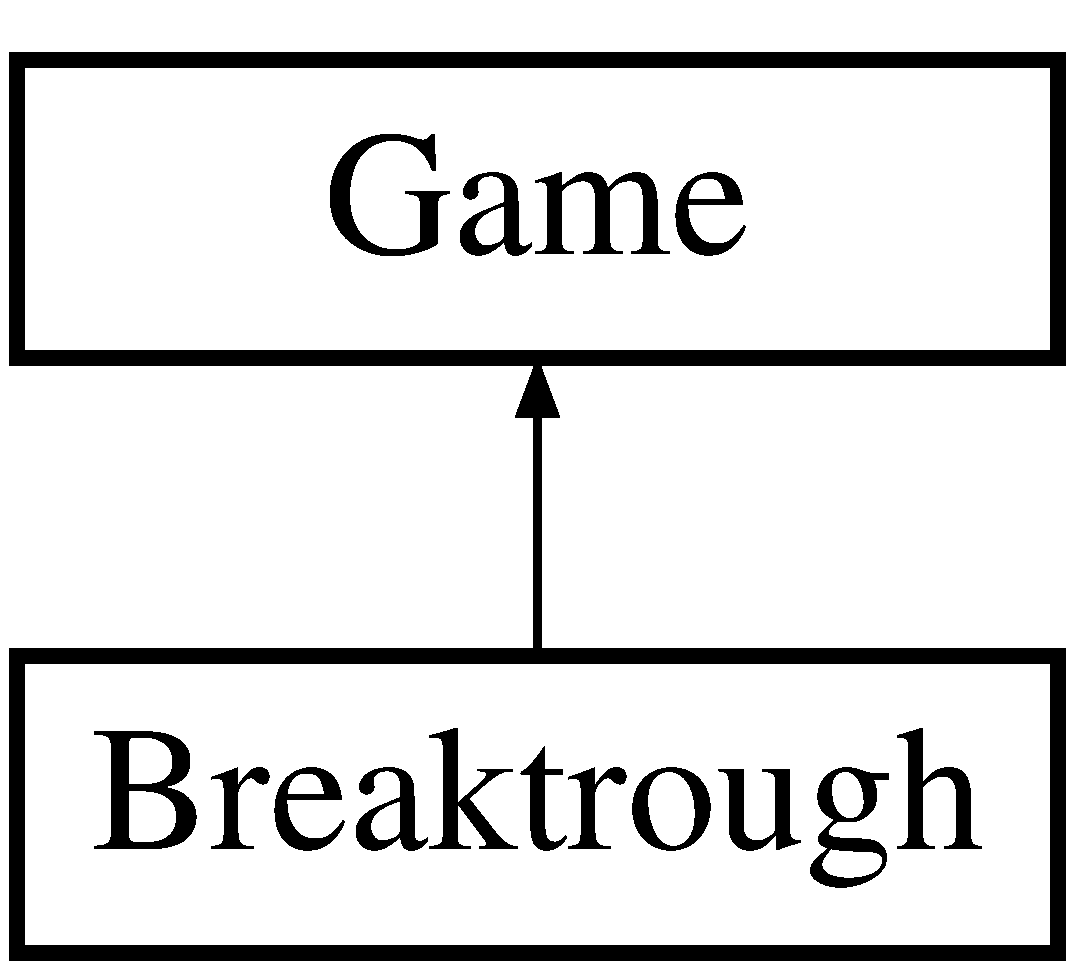
\includegraphics[height=2.000000cm]{class_breaktrough}
\end{center}
\end{figure}
\subsection*{Public Member Functions}
\begin{DoxyCompactItemize}
\item 
\hyperlink{class_breaktrough_a988083f0722bff1058a980748c65705f}{Breaktrough} ()
\begin{DoxyCompactList}\small\item\em $<$ Default Breaktrhough game constructor \end{DoxyCompactList}\item 
void \hyperlink{class_breaktrough_a1e1244669a6ab63043329afcdaaeec37}{set\-Move\-For\-Player} (int P)
\item 
virtual void \hyperlink{class_breaktrough_a07006aa5d9919ddefa68554f3022afc6}{make} (int From\-X, int From\-Y, int To\-X, int To\-Y)
\begin{DoxyCompactList}\small\item\em $<$ Make move from current cord to dest cord \end{DoxyCompactList}\item 
\hypertarget{class_breaktrough_a1e4b2c80e074f7052c4c491abe95c9f6}{virtual void \hyperlink{class_breaktrough_a1e4b2c80e074f7052c4c491abe95c9f6}{start} ()}\label{class_breaktrough_a1e4b2c80e074f7052c4c491abe95c9f6}

\begin{DoxyCompactList}\small\item\em Get legal moves for piece, returns up to 3 legal cords depending on position. Front, Front\-Right, and Front\-Left. \end{DoxyCompactList}\item 
void \hyperlink{class_breaktrough_a6bf5d444ace61244df9a0255fde5d533}{legal} (vector$<$ \hyperlink{struct_point}{Point} $>$ \&legal\-Moves, \hyperlink{class_piece}{Piece} \&piece)
\begin{DoxyCompactList}\small\item\em Check if game has ended. \end{DoxyCompactList}\item 
\hypertarget{class_breaktrough_ae9e5edbac2c2fcce47711697eb3a8a2d}{virtual void {\bfseries check\-Finished} ()}\label{class_breaktrough_ae9e5edbac2c2fcce47711697eb3a8a2d}

\end{DoxyCompactItemize}
\subsection*{Additional Inherited Members}


\subsection{Constructor \& Destructor Documentation}
\hypertarget{class_breaktrough_a988083f0722bff1058a980748c65705f}{\index{Breaktrough@{Breaktrough}!Breaktrough@{Breaktrough}}
\index{Breaktrough@{Breaktrough}!Breaktrough@{Breaktrough}}
\subsubsection[{Breaktrough}]{\setlength{\rightskip}{0pt plus 5cm}Breaktrough\-::\-Breaktrough (
\begin{DoxyParamCaption}
{}
\end{DoxyParamCaption}
)}}\label{class_breaktrough_a988083f0722bff1058a980748c65705f}


$<$ Default Breaktrhough game constructor 

initialize pieces for players and set distance for moves for each direction 

\subsection{Member Function Documentation}
\hypertarget{class_breaktrough_a6bf5d444ace61244df9a0255fde5d533}{\index{Breaktrough@{Breaktrough}!legal@{legal}}
\index{legal@{legal}!Breaktrough@{Breaktrough}}
\subsubsection[{legal}]{\setlength{\rightskip}{0pt plus 5cm}void Breaktrough\-::legal (
\begin{DoxyParamCaption}
\item[{vector$<$ {\bf Point} $>$ \&}]{legal\-Moves, }
\item[{{\bf Piece} \&}]{piece}
\end{DoxyParamCaption}
)\hspace{0.3cm}{\ttfamily [virtual]}}}\label{class_breaktrough_a6bf5d444ace61244df9a0255fde5d533}


Check if game has ended. 


\begin{DoxyParams}{Parameters}
{\em \&legal\-Moves} & reference to result vector \\
\hline
{\em \&piece} & reference to piece being moved \\
\hline
\end{DoxyParams}


Reimplemented from \hyperlink{class_game_acf61b27aed22684d96fbc7fa2692feeb}{Game}.

\hypertarget{class_breaktrough_a07006aa5d9919ddefa68554f3022afc6}{\index{Breaktrough@{Breaktrough}!make@{make}}
\index{make@{make}!Breaktrough@{Breaktrough}}
\subsubsection[{make}]{\setlength{\rightskip}{0pt plus 5cm}void Breaktrough\-::make (
\begin{DoxyParamCaption}
\item[{int}]{From\-X, }
\item[{int}]{From\-Y, }
\item[{int}]{To\-X, }
\item[{int}]{To\-Y}
\end{DoxyParamCaption}
)\hspace{0.3cm}{\ttfamily [virtual]}}}\label{class_breaktrough_a07006aa5d9919ddefa68554f3022afc6}


$<$ Make move from current cord to dest cord 


\begin{DoxyParams}{Parameters}
{\em From\-X} & cord \\
\hline
{\em From\-Y} & cord \\
\hline
{\em To\-X} & cord \\
\hline
{\em To\-Y} & cord\-Initialize and starta game Breakthrough \\
\hline
\end{DoxyParams}


Reimplemented from \hyperlink{class_game_a50b3e0e1e7a73793a9f9eae1b0660eff}{Game}.

\hypertarget{class_breaktrough_a1e1244669a6ab63043329afcdaaeec37}{\index{Breaktrough@{Breaktrough}!set\-Move\-For\-Player@{set\-Move\-For\-Player}}
\index{set\-Move\-For\-Player@{set\-Move\-For\-Player}!Breaktrough@{Breaktrough}}
\subsubsection[{set\-Move\-For\-Player}]{\setlength{\rightskip}{0pt plus 5cm}void Breaktrough\-::set\-Move\-For\-Player (
\begin{DoxyParamCaption}
\item[{int}]{P}
\end{DoxyParamCaption}
)}}\label{class_breaktrough_a1e1244669a6ab63043329afcdaaeec37}

\begin{DoxyParams}{Parameters}
{\em P} & indicates what player, 0=player1 and 1 = player2 \\
\hline
\end{DoxyParams}


The documentation for this class was generated from the following files\-:\begin{DoxyCompactItemize}
\item 
Breakthrough.\-h\item 
Breakthrough.\-cpp\end{DoxyCompactItemize}

\hypertarget{class_game}{\section{Game Class Reference}
\label{class_game}\index{Game@{Game}}
}


Brief description. Class \hyperlink{class_game}{Game} use as base interface for 2 player board games.  




{\ttfamily \#include $<$Game.\-h$>$}

Inheritance diagram for Game\-:\begin{figure}[H]
\begin{center}
\leavevmode
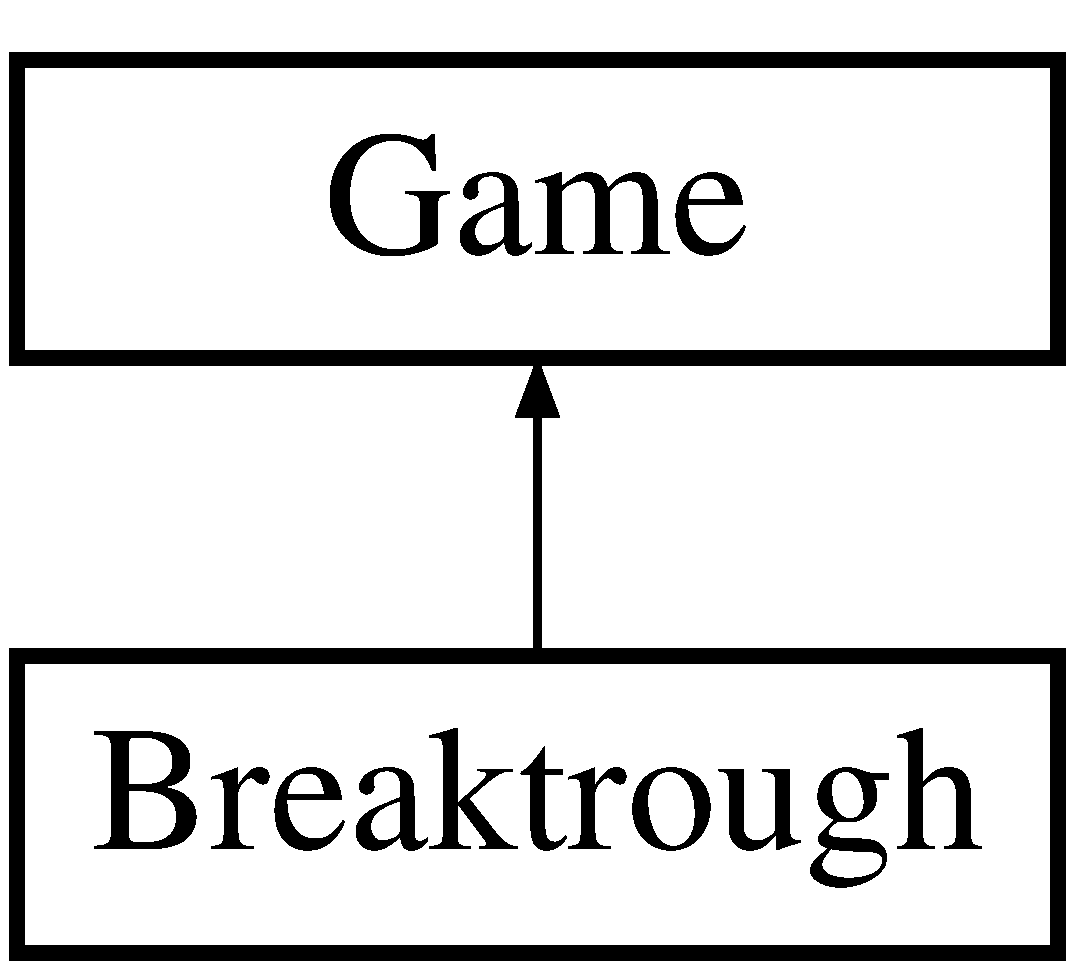
\includegraphics[height=2.000000cm]{class_game}
\end{center}
\end{figure}
\subsection*{Public Member Functions}
\begin{DoxyCompactItemize}
\item 
\hyperlink{class_game_ad59df6562a58a614fda24622d3715b65}{Game} ()
\begin{DoxyCompactList}\small\item\em $<$ Default \hyperlink{class_game}{Game} constructor \end{DoxyCompactList}\item 
virtual void \hyperlink{class_game_acf61b27aed22684d96fbc7fa2692feeb}{legal} (vector$<$ \hyperlink{struct_point}{Point} $>$ \&legal\-Moves, \hyperlink{class_piece}{Piece} \&piece)
\item 
virtual void \hyperlink{class_game_a3d9b98f7c4a96ecf578f75b96c9f0e90}{start} ()
\begin{DoxyCompactList}\small\item\em Virtual void to start game. \end{DoxyCompactList}\item 
virtual void \hyperlink{class_game_a50b3e0e1e7a73793a9f9eae1b0660eff}{make} (int From\-X, int From\-Y, int To\-X, int To\-Y)
\item 
\hypertarget{class_game_ab411d0da584724addd4fdb96fc16b9a4}{virtual void \hyperlink{class_game_ab411d0da584724addd4fdb96fc16b9a4}{go} ()}\label{class_game_ab411d0da584724addd4fdb96fc16b9a4}

\begin{DoxyCompactList}\small\item\em Virtual void function to let cpu make move according to difficult level. \end{DoxyCompactList}\item 
\hypertarget{class_game_a9be0655102af94f1a37a7eaec1be36fc}{void \hyperlink{class_game_a9be0655102af94f1a37a7eaec1be36fc}{retract} ()}\label{class_game_a9be0655102af94f1a37a7eaec1be36fc}

\begin{DoxyCompactList}\small\item\em Retract last move, pops Game\-Board state and sets game to last state. \end{DoxyCompactList}\item 
\hypertarget{class_game_a4d0223a84926cbabea95ed7e0392690a}{virtual void \hyperlink{class_game_a4d0223a84926cbabea95ed7e0392690a}{display} ()}\label{class_game_a4d0223a84926cbabea95ed7e0392690a}

\begin{DoxyCompactList}\small\item\em Display board. \end{DoxyCompactList}\item 
\hypertarget{class_game_a3bc8822cacd9cf8c5f71021072eb24a4}{virtual void \hyperlink{class_game_a3bc8822cacd9cf8c5f71021072eb24a4}{evaluate} ()}\label{class_game_a3bc8822cacd9cf8c5f71021072eb24a4}

\begin{DoxyCompactList}\small\item\em Virtual void, evaluate if player can make move in current position and set score. \end{DoxyCompactList}\item 
\hypertarget{class_game_a29997a321e10a5456f0aef9e95c51757}{void \hyperlink{class_game_a29997a321e10a5456f0aef9e95c51757}{debug} ()}\label{class_game_a29997a321e10a5456f0aef9e95c51757}

\begin{DoxyCompactList}\small\item\em Switch between debug mode and non-\/debug mode. \end{DoxyCompactList}\item 
\hypertarget{class_game_a8272be134d16c277bb014ad6a22fc357}{void \hyperlink{class_game_a8272be134d16c277bb014ad6a22fc357}{quit} ()}\label{class_game_a8272be134d16c277bb014ad6a22fc357}

\begin{DoxyCompactList}\small\item\em Exit program. \end{DoxyCompactList}\item 
\hypertarget{class_game_ab81299d944d2779d482067640e576389}{string \hyperlink{class_game_ab81299d944d2779d482067640e576389}{Get\-Name} ()}\label{class_game_ab81299d944d2779d482067640e576389}

\begin{DoxyCompactList}\small\item\em Returns name. \end{DoxyCompactList}\item 
\hypertarget{class_game_ae8ac0005c039f0f5f2dd1c10a299fe8d}{void \hyperlink{class_game_ae8ac0005c039f0f5f2dd1c10a299fe8d}{set\-Difficulty} (int diff)}\label{class_game_ae8ac0005c039f0f5f2dd1c10a299fe8d}

\begin{DoxyCompactList}\small\item\em Sets difficult state 0 = random, 1 = easy, 2 = medium, 3 = hard. \end{DoxyCompactList}\item 
\hypertarget{class_game_a2c0efe888e453a7fc0e644503fbd6316}{int \hyperlink{class_game_a2c0efe888e453a7fc0e644503fbd6316}{get\-Difficulty} ()}\label{class_game_a2c0efe888e453a7fc0e644503fbd6316}

\begin{DoxyCompactList}\small\item\em Returns current difficulty level. \end{DoxyCompactList}\item 
\hypertarget{class_game_a1f47238d93728540edb7940a80a9db89}{void \hyperlink{class_game_a1f47238d93728540edb7940a80a9db89}{Get\-Test\-Game} ()}\label{class_game_a1f47238d93728540edb7940a80a9db89}

\begin{DoxyCompactList}\small\item\em Runs Test game. \end{DoxyCompactList}\item 
\hypertarget{class_game_ae5be70ea28f2ec151cd93e86086f23a9}{void \hyperlink{class_game_ae5be70ea28f2ec151cd93e86086f23a9}{check\-Finished} ()}\label{class_game_ae5be70ea28f2ec151cd93e86086f23a9}

\begin{DoxyCompactList}\small\item\em Prints out result if game has finished. \end{DoxyCompactList}\item 
\hypertarget{class_game_a37edad1c1ded84b1735653f809ccb585}{bool \hyperlink{class_game_a37edad1c1ded84b1735653f809ccb585}{can\-Make} (\hyperlink{class_piece}{Piece} $\ast$piece, \hyperlink{struct_point}{Point} p)}\label{class_game_a37edad1c1ded84b1735653f809ccb585}

\begin{DoxyCompactList}\small\item\em Cheks if piece can make move to cord p. \end{DoxyCompactList}\end{DoxyCompactItemize}
\subsection*{Public Attributes}
\begin{DoxyCompactItemize}
\item 
bool \hyperlink{class_game_aee0b70deb19422d35b2061beb339bdf8}{m\-\_\-finished}
\item 
bool \hyperlink{class_game_ad79740c2d2fa299cf322bf6ea322d9aa}{Debug}
\item 
\hyperlink{class_board}{Board} \hyperlink{class_game_aeb67bc4fc06221330cfd7c862c85b66d}{Game\-Board}
\end{DoxyCompactItemize}
\subsection*{Protected Attributes}
\begin{DoxyCompactItemize}
\item 
string \hyperlink{class_game_a1b56d5db37d900da0911378cc01f4cad}{Game\-Name}
\item 
int \hyperlink{class_game_aea2c7f8bdb891f32026750c81f6eac16}{player1\-\_\-pieces}
\item 
int \hyperlink{class_game_a2b82ab082220d93bab2d7d1d181ad639}{player2\-\_\-pieces}
\item 
int \hyperlink{class_game_a536a6390d16f05d402928bd731e06ef3}{difficulty}
\item 
vector$<$ \hyperlink{class_board}{Board} $>$ \hyperlink{class_game_a7c0dd74fa2e5c366638596b7e82428f1}{history}
\item 
int \hyperlink{class_game_a53cb9be6604469db6b3abac24c5a2ab6}{Max\-Plays}
\item 
int \hyperlink{class_game_a88700a4643e08b12130ba2950c54ed8b}{Current\-Turn}
\item 
int \hyperlink{class_game_a661282d67a0e4a972293c98478bc02e4}{Current\-Player}
\end{DoxyCompactItemize}


\subsection{Detailed Description}
Brief description. Class \hyperlink{class_game}{Game} use as base interface for 2 player board games. 

\hyperlink{class_game}{Game} class is used as parent class for each type of boardgames. The class has some basic default actions. 

\subsection{Constructor \& Destructor Documentation}
\hypertarget{class_game_ad59df6562a58a614fda24622d3715b65}{\index{Game@{Game}!Game@{Game}}
\index{Game@{Game}!Game@{Game}}
\subsubsection[{Game}]{\setlength{\rightskip}{0pt plus 5cm}Game\-::\-Game (
\begin{DoxyParamCaption}
{}
\end{DoxyParamCaption}
)}}\label{class_game_ad59df6562a58a614fda24622d3715b65}


$<$ Default \hyperlink{class_game}{Game} constructor 

Virtual void, returns legal moves for piece in current game with moves ref 

\subsection{Member Function Documentation}
\hypertarget{class_game_acf61b27aed22684d96fbc7fa2692feeb}{\index{Game@{Game}!legal@{legal}}
\index{legal@{legal}!Game@{Game}}
\subsubsection[{legal}]{\setlength{\rightskip}{0pt plus 5cm}virtual void Game\-::legal (
\begin{DoxyParamCaption}
\item[{vector$<$ {\bf Point} $>$ \&}]{legal\-Moves, }
\item[{{\bf Piece} \&}]{piece}
\end{DoxyParamCaption}
)\hspace{0.3cm}{\ttfamily [inline]}, {\ttfamily [virtual]}}}\label{class_game_acf61b27aed22684d96fbc7fa2692feeb}

\begin{DoxyParams}{Parameters}
{\em \&legal\-Moves} & a reference to vector of \hyperlink{struct_point}{Point}. Returns legal moves in vector \\
\hline
{\em \&piece} & a reference to piece being moved \\
\hline
\end{DoxyParams}
\begin{DoxyReturn}{Returns}
The test results 
\end{DoxyReturn}


Reimplemented in \hyperlink{class_breaktrough_a6bf5d444ace61244df9a0255fde5d533}{Breaktrough}.

\hypertarget{class_game_a50b3e0e1e7a73793a9f9eae1b0660eff}{\index{Game@{Game}!make@{make}}
\index{make@{make}!Game@{Game}}
\subsubsection[{make}]{\setlength{\rightskip}{0pt plus 5cm}void Game\-::make (
\begin{DoxyParamCaption}
\item[{int}]{From\-X, }
\item[{int}]{From\-Y, }
\item[{int}]{To\-X, }
\item[{int}]{To\-Y}
\end{DoxyParamCaption}
)\hspace{0.3cm}{\ttfamily [virtual]}}}\label{class_game_a50b3e0e1e7a73793a9f9eae1b0660eff}

\begin{DoxyParams}{Parameters}
{\em From\-X} & x value for piece to be moved \\
\hline
{\em From\-Y} & y value for piece to be moved \\
\hline
{\em To\-X} & x value for destination \\
\hline
{\em To\-Y} & y value for destination \\
\hline
\end{DoxyParams}


Reimplemented in \hyperlink{class_breaktrough_a07006aa5d9919ddefa68554f3022afc6}{Breaktrough}.

\hypertarget{class_game_a3d9b98f7c4a96ecf578f75b96c9f0e90}{\index{Game@{Game}!start@{start}}
\index{start@{start}!Game@{Game}}
\subsubsection[{start}]{\setlength{\rightskip}{0pt plus 5cm}void Game\-::start (
\begin{DoxyParamCaption}
{}
\end{DoxyParamCaption}
)\hspace{0.3cm}{\ttfamily [virtual]}}}\label{class_game_a3d9b98f7c4a96ecf578f75b96c9f0e90}


Virtual void to start game. 

Virtual void to make move, move 1 piece from cord to other cord 

Reimplemented in \hyperlink{class_breaktrough_a1e4b2c80e074f7052c4c491abe95c9f6}{Breaktrough}.



\subsection{Member Data Documentation}
\hypertarget{class_game_a661282d67a0e4a972293c98478bc02e4}{\index{Game@{Game}!Current\-Player@{Current\-Player}}
\index{Current\-Player@{Current\-Player}!Game@{Game}}
\subsubsection[{Current\-Player}]{\setlength{\rightskip}{0pt plus 5cm}int Game\-::\-Current\-Player\hspace{0.3cm}{\ttfamily [protected]}}}\label{class_game_a661282d67a0e4a972293c98478bc02e4}
Indicates who´s player turn it is \hypertarget{class_game_a88700a4643e08b12130ba2950c54ed8b}{\index{Game@{Game}!Current\-Turn@{Current\-Turn}}
\index{Current\-Turn@{Current\-Turn}!Game@{Game}}
\subsubsection[{Current\-Turn}]{\setlength{\rightskip}{0pt plus 5cm}int Game\-::\-Current\-Turn\hspace{0.3cm}{\ttfamily [protected]}}}\label{class_game_a88700a4643e08b12130ba2950c54ed8b}
Keeps current move, counts each move \hypertarget{class_game_ad79740c2d2fa299cf322bf6ea322d9aa}{\index{Game@{Game}!Debug@{Debug}}
\index{Debug@{Debug}!Game@{Game}}
\subsubsection[{Debug}]{\setlength{\rightskip}{0pt plus 5cm}bool Game\-::\-Debug}}\label{class_game_ad79740c2d2fa299cf322bf6ea322d9aa}
Toggle switch for debugging, if true program prints debug info \hypertarget{class_game_a536a6390d16f05d402928bd731e06ef3}{\index{Game@{Game}!difficulty@{difficulty}}
\index{difficulty@{difficulty}!Game@{Game}}
\subsubsection[{difficulty}]{\setlength{\rightskip}{0pt plus 5cm}int Game\-::difficulty\hspace{0.3cm}{\ttfamily [protected]}}}\label{class_game_a536a6390d16f05d402928bd731e06ef3}
Keeps difficulty level \hypertarget{class_game_aeb67bc4fc06221330cfd7c862c85b66d}{\index{Game@{Game}!Game\-Board@{Game\-Board}}
\index{Game\-Board@{Game\-Board}!Game@{Game}}
\subsubsection[{Game\-Board}]{\setlength{\rightskip}{0pt plus 5cm}{\bf Board} Game\-::\-Game\-Board}}\label{class_game_aeb67bc4fc06221330cfd7c862c85b66d}
\hyperlink{class_game}{Game} instance of class Game\-Board \hypertarget{class_game_a1b56d5db37d900da0911378cc01f4cad}{\index{Game@{Game}!Game\-Name@{Game\-Name}}
\index{Game\-Name@{Game\-Name}!Game@{Game}}
\subsubsection[{Game\-Name}]{\setlength{\rightskip}{0pt plus 5cm}string Game\-::\-Game\-Name\hspace{0.3cm}{\ttfamily [protected]}}}\label{class_game_a1b56d5db37d900da0911378cc01f4cad}
Name of the game \hypertarget{class_game_a7c0dd74fa2e5c366638596b7e82428f1}{\index{Game@{Game}!history@{history}}
\index{history@{history}!Game@{Game}}
\subsubsection[{history}]{\setlength{\rightskip}{0pt plus 5cm}vector$<${\bf Board}$>$ Game\-::history\hspace{0.3cm}{\ttfamily [protected]}}}\label{class_game_a7c0dd74fa2e5c366638596b7e82428f1}
Vector of each game state, changes each turn \hypertarget{class_game_aee0b70deb19422d35b2061beb339bdf8}{\index{Game@{Game}!m\-\_\-finished@{m\-\_\-finished}}
\index{m\-\_\-finished@{m\-\_\-finished}!Game@{Game}}
\subsubsection[{m\-\_\-finished}]{\setlength{\rightskip}{0pt plus 5cm}bool Game\-::m\-\_\-finished}}\label{class_game_aee0b70deb19422d35b2061beb339bdf8}
Indicates if still possible to make moves or if game has finished \hypertarget{class_game_a53cb9be6604469db6b3abac24c5a2ab6}{\index{Game@{Game}!Max\-Plays@{Max\-Plays}}
\index{Max\-Plays@{Max\-Plays}!Game@{Game}}
\subsubsection[{Max\-Plays}]{\setlength{\rightskip}{0pt plus 5cm}int Game\-::\-Max\-Plays\hspace{0.3cm}{\ttfamily [protected]}}}\label{class_game_a53cb9be6604469db6b3abac24c5a2ab6}
Keeps max moves in game \hypertarget{class_game_aea2c7f8bdb891f32026750c81f6eac16}{\index{Game@{Game}!player1\-\_\-pieces@{player1\-\_\-pieces}}
\index{player1\-\_\-pieces@{player1\-\_\-pieces}!Game@{Game}}
\subsubsection[{player1\-\_\-pieces}]{\setlength{\rightskip}{0pt plus 5cm}int Game\-::player1\-\_\-pieces\hspace{0.3cm}{\ttfamily [protected]}}}\label{class_game_aea2c7f8bdb891f32026750c81f6eac16}
Amount of pieces for player 1 \hypertarget{class_game_a2b82ab082220d93bab2d7d1d181ad639}{\index{Game@{Game}!player2\-\_\-pieces@{player2\-\_\-pieces}}
\index{player2\-\_\-pieces@{player2\-\_\-pieces}!Game@{Game}}
\subsubsection[{player2\-\_\-pieces}]{\setlength{\rightskip}{0pt plus 5cm}int Game\-::player2\-\_\-pieces\hspace{0.3cm}{\ttfamily [protected]}}}\label{class_game_a2b82ab082220d93bab2d7d1d181ad639}
Amount of pieces for player 2 

The documentation for this class was generated from the following files\-:\begin{DoxyCompactItemize}
\item 
Game.\-h\item 
Game.\-cpp\end{DoxyCompactItemize}

\hypertarget{struct_move_dir}{\section{Move\-Dir Struct Reference}
\label{struct_move_dir}\index{Move\-Dir@{Move\-Dir}}
}


Brief description. Simple struct that indicats how far a piece can move each turn for each direction.  




{\ttfamily \#include $<$Pieces.\-h$>$}

\subsection*{Public Attributes}
\begin{DoxyCompactItemize}
\item 
\hypertarget{struct_move_dir_abf2617e5000f6d25e8dfe0d9cb41d5ab}{int {\bfseries N}}\label{struct_move_dir_abf2617e5000f6d25e8dfe0d9cb41d5ab}

\item 
\hypertarget{struct_move_dir_a2373da17371963eab23101b4eef0d40e}{int {\bfseries E}}\label{struct_move_dir_a2373da17371963eab23101b4eef0d40e}

\item 
\hypertarget{struct_move_dir_a02ef68f2e799daf66a82a0d9318fc2fb}{int {\bfseries S}}\label{struct_move_dir_a02ef68f2e799daf66a82a0d9318fc2fb}

\item 
\hypertarget{struct_move_dir_ae7d3fc3e4f692079d3848bff650f6edd}{int {\bfseries W}}\label{struct_move_dir_ae7d3fc3e4f692079d3848bff650f6edd}

\end{DoxyCompactItemize}


\subsection{Detailed Description}
Brief description. Simple struct that indicats how far a piece can move each turn for each direction. 

The documentation for this struct was generated from the following file\-:\begin{DoxyCompactItemize}
\item 
Pieces.\-h\end{DoxyCompactItemize}

\hypertarget{class_pawn}{\section{Pawn Class Reference}
\label{class_pawn}\index{Pawn@{Pawn}}
}
Inheritance diagram for Pawn\-:\begin{figure}[H]
\begin{center}
\leavevmode
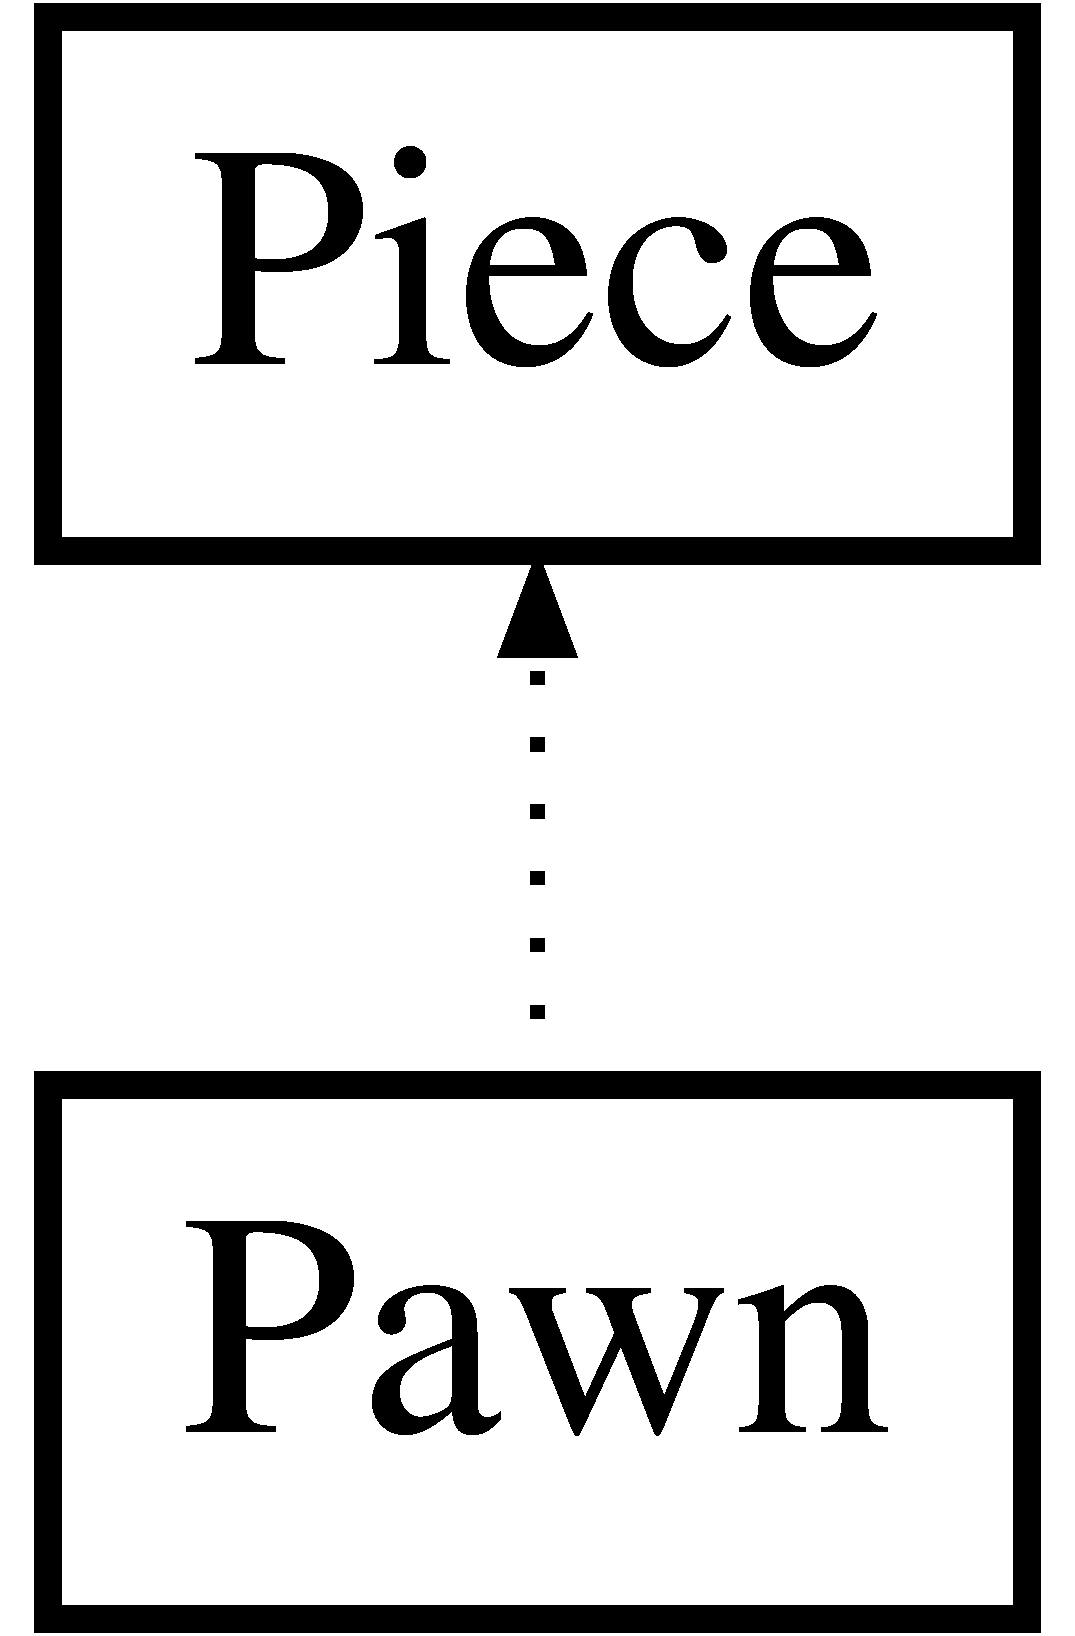
\includegraphics[height=2.000000cm]{class_pawn}
\end{center}
\end{figure}
\subsection*{Public Member Functions}
\begin{DoxyCompactItemize}
\item 
virtual void \hyperlink{class_pawn_ab08f4e1682965a0a251c60a9857685bf}{get\-Moves} (std\-::vector$<$ \hyperlink{struct_point}{Point} $>$ \&points, const int board\-Size)
\end{DoxyCompactItemize}
\subsection*{Additional Inherited Members}


\subsection{Member Function Documentation}
\hypertarget{class_pawn_ab08f4e1682965a0a251c60a9857685bf}{\index{Pawn@{Pawn}!get\-Moves@{get\-Moves}}
\index{get\-Moves@{get\-Moves}!Pawn@{Pawn}}
\subsubsection[{get\-Moves}]{\setlength{\rightskip}{0pt plus 5cm}void Pawn\-::get\-Moves (
\begin{DoxyParamCaption}
\item[{std\-::vector$<$ {\bf Point} $>$ \&}]{points, }
\item[{const int}]{board\-Size}
\end{DoxyParamCaption}
)\hspace{0.3cm}{\ttfamily [virtual]}}}\label{class_pawn_ab08f4e1682965a0a251c60a9857685bf}
if player = 1 

Reimplemented from \hyperlink{class_piece}{Piece}.



The documentation for this class was generated from the following files\-:\begin{DoxyCompactItemize}
\item 
Pawn.\-h\item 
Pawn.\-cpp\end{DoxyCompactItemize}

\hypertarget{class_piece}{\section{Piece Class Reference}
\label{class_piece}\index{Piece@{Piece}}
}
Inheritance diagram for Piece\-:\begin{figure}[H]
\begin{center}
\leavevmode
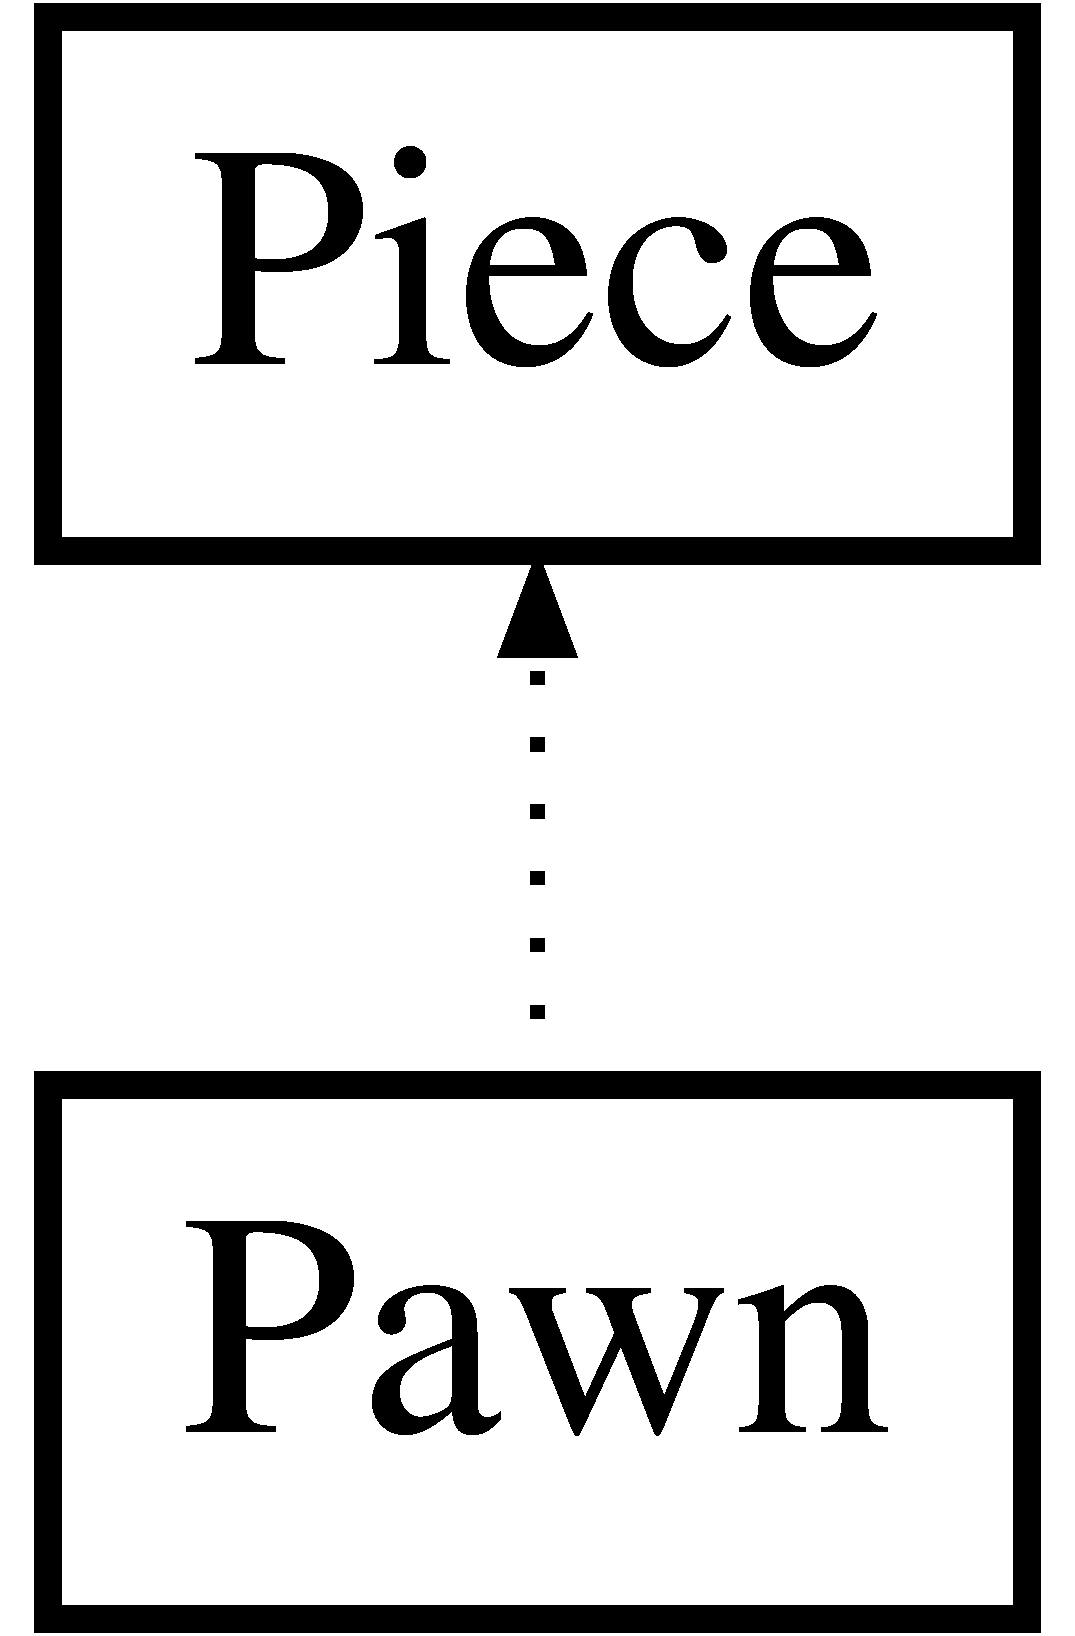
\includegraphics[height=2.000000cm]{class_piece}
\end{center}
\end{figure}
\subsection*{Public Member Functions}
\begin{DoxyCompactItemize}
\item 
\hypertarget{class_piece_af20b3f54c1dfafe3aac36bac2a0cafaf}{{\bfseries Piece} (char $\ast$type, int player\-Number, \hyperlink{struct_point}{Point} position)}\label{class_piece_af20b3f54c1dfafe3aac36bac2a0cafaf}

\item 
\hypertarget{class_piece_af0360ba66c38dc5f35b0de53653c0136}{virtual void {\bfseries move} (\hyperlink{struct_point}{Point} p)}\label{class_piece_af0360ba66c38dc5f35b0de53653c0136}

\item 
\hypertarget{class_piece_a84ba6ffb15c8e35be6a2eaa768a79d8c}{virtual void {\bfseries set\-Player} (int p)}\label{class_piece_a84ba6ffb15c8e35be6a2eaa768a79d8c}

\item 
\hypertarget{class_piece_aed124504a141b5920baf6919d7aa07a1}{virtual void {\bfseries set\-Moves} (int dir\-N, int dir\-E, int dir\-S, int dir\-W)}\label{class_piece_aed124504a141b5920baf6919d7aa07a1}

\item 
\hypertarget{class_piece_a24d8dbf44002666b0cdbc82c3fe689c3}{virtual void {\bfseries get\-Moves} (std\-::vector$<$ \hyperlink{struct_point}{Point} $>$ \&points, const int board\-Size)}\label{class_piece_a24d8dbf44002666b0cdbc82c3fe689c3}

\item 
\hypertarget{class_piece_a72665a008584e735f6c04ce91038c7e4}{void {\bfseries set\-Position} (int x, int y)}\label{class_piece_a72665a008584e735f6c04ce91038c7e4}

\item 
\hypertarget{class_piece_a016d7fe7de3eda5e10ea1a0bda8900e8}{void {\bfseries set\-Position} (\hyperlink{struct_point}{Point} p)}\label{class_piece_a016d7fe7de3eda5e10ea1a0bda8900e8}

\item 
\hypertarget{class_piece_a6f756ed0481304973757272233addbd4}{void {\bfseries print} ()}\label{class_piece_a6f756ed0481304973757272233addbd4}

\item 
\hypertarget{class_piece_ab011e4ae76a47c8f5a57fed6ed3bc40c}{\hyperlink{struct_point}{Point} {\bfseries get\-Postion} ()}\label{class_piece_ab011e4ae76a47c8f5a57fed6ed3bc40c}

\item 
\hypertarget{class_piece_ae3ab3d26428b104eea1ef049c0b65f3a}{\hyperlink{struct_move_dir}{Move\-Dir} {\bfseries get\-Mov\-Dir} ()}\label{class_piece_ae3ab3d26428b104eea1ef049c0b65f3a}

\item 
\hypertarget{class_piece_ab1aefb3821698fb08fd6eafd5e4c8f5a}{bool {\bfseries get\-Has\-Moved} ()}\label{class_piece_ab1aefb3821698fb08fd6eafd5e4c8f5a}

\item 
\hypertarget{class_piece_acc0b7c99053c361cd55f0231e3b6e272}{int {\bfseries get\-Player} ()}\label{class_piece_acc0b7c99053c361cd55f0231e3b6e272}

\item 
\hypertarget{class_piece_a39392c919bff7c404cc05b6b31e6bf32}{char $\ast$ {\bfseries get\-Type} ()}\label{class_piece_a39392c919bff7c404cc05b6b31e6bf32}

\end{DoxyCompactItemize}


The documentation for this class was generated from the following files\-:\begin{DoxyCompactItemize}
\item 
Pieces.\-h\item 
Pieces.\-cpp\end{DoxyCompactItemize}

\hypertarget{struct_point}{\section{Point Struct Reference}
\label{struct_point}\index{Point@{Point}}
}


Brief description. struct \hyperlink{struct_point}{Point} simple struct for cords, implements comparision between \hyperlink{struct_point}{Point} instances and assigning values.  




{\ttfamily \#include $<$Pieces.\-h$>$}

\subsection*{Public Member Functions}
\begin{DoxyCompactItemize}
\item 
\hyperlink{struct_point_a001c4958c310b248f5c26037aea38a9c}{Point} (int x, int y)
\begin{DoxyCompactList}\small\item\em default constructor \end{DoxyCompactList}\item 
\hypertarget{struct_point_a26844fd8368a6c5d34713d8ac1185fbe}{void {\bfseries set\-Empty} ()}\label{struct_point_a26844fd8368a6c5d34713d8ac1185fbe}

\item 
\hypertarget{struct_point_a76c5855c06d98aed16b5796a9a50bbee}{void \hyperlink{struct_point_a76c5855c06d98aed16b5796a9a50bbee}{print} ()}\label{struct_point_a76c5855c06d98aed16b5796a9a50bbee}

\begin{DoxyCompactList}\small\item\em Sets cord x and y values to 0. \end{DoxyCompactList}\item 
\hypertarget{struct_point_a5bb149491b3759746415a8ed97d63d25}{void {\bfseries operator=} (const \hyperlink{struct_point}{Point} \&rhs)}\label{struct_point_a5bb149491b3759746415a8ed97d63d25}

\end{DoxyCompactItemize}
\subsection*{Public Attributes}
\begin{DoxyCompactItemize}
\item 
\hypertarget{struct_point_a885daee8c5064cd51f6a4c3888091fc9}{int \hyperlink{struct_point_a885daee8c5064cd51f6a4c3888091fc9}{m\-\_\-x}}\label{struct_point_a885daee8c5064cd51f6a4c3888091fc9}

\begin{DoxyCompactList}\small\item\em x value for cord \end{DoxyCompactList}\item 
\hypertarget{struct_point_a00e243381d01e186dc2fcc5d24b4d3be}{int \hyperlink{struct_point_a00e243381d01e186dc2fcc5d24b4d3be}{m\-\_\-y}}\label{struct_point_a00e243381d01e186dc2fcc5d24b4d3be}

\begin{DoxyCompactList}\small\item\em y value for cord \end{DoxyCompactList}\end{DoxyCompactItemize}
\subsection*{Friends}
\begin{DoxyCompactItemize}
\item 
\hypertarget{struct_point_a75de5fa7971bc4ffdd3c5d06d776495c}{bool \hyperlink{struct_point_a75de5fa7971bc4ffdd3c5d06d776495c}{operator==} (\hyperlink{struct_point}{Point} \&lhs, \hyperlink{struct_point}{Point} \&rhs)}\label{struct_point_a75de5fa7971bc4ffdd3c5d06d776495c}

\begin{DoxyCompactList}\small\item\em prints out cordination as \char`\"{}(x, y)\char`\"{} \end{DoxyCompactList}\end{DoxyCompactItemize}


\subsection{Detailed Description}
Brief description. struct \hyperlink{struct_point}{Point} simple struct for cords, implements comparision between \hyperlink{struct_point}{Point} instances and assigning values. 

\subsection{Constructor \& Destructor Documentation}
\hypertarget{struct_point_a001c4958c310b248f5c26037aea38a9c}{\index{Point@{Point}!Point@{Point}}
\index{Point@{Point}!Point@{Point}}
\subsubsection[{Point}]{\setlength{\rightskip}{0pt plus 5cm}Point\-::\-Point (
\begin{DoxyParamCaption}
\item[{int}]{x, }
\item[{int}]{y}
\end{DoxyParamCaption}
)\hspace{0.3cm}{\ttfamily [inline]}}}\label{struct_point_a001c4958c310b248f5c26037aea38a9c}


default constructor 

Constructor that takes cors as parameter and sets values


\begin{DoxyParams}{Parameters}
{\em x} & X value for cord \\
\hline
{\em y} & Y value for cord \\
\hline
\end{DoxyParams}


The documentation for this struct was generated from the following file\-:\begin{DoxyCompactItemize}
\item 
Pieces.\-h\end{DoxyCompactItemize}

\hypertarget{class_test_game}{\section{Test\-Game Class Reference}
\label{class_test_game}\index{Test\-Game@{Test\-Game}}
}
Inheritance diagram for Test\-Game\-:\begin{figure}[H]
\begin{center}
\leavevmode
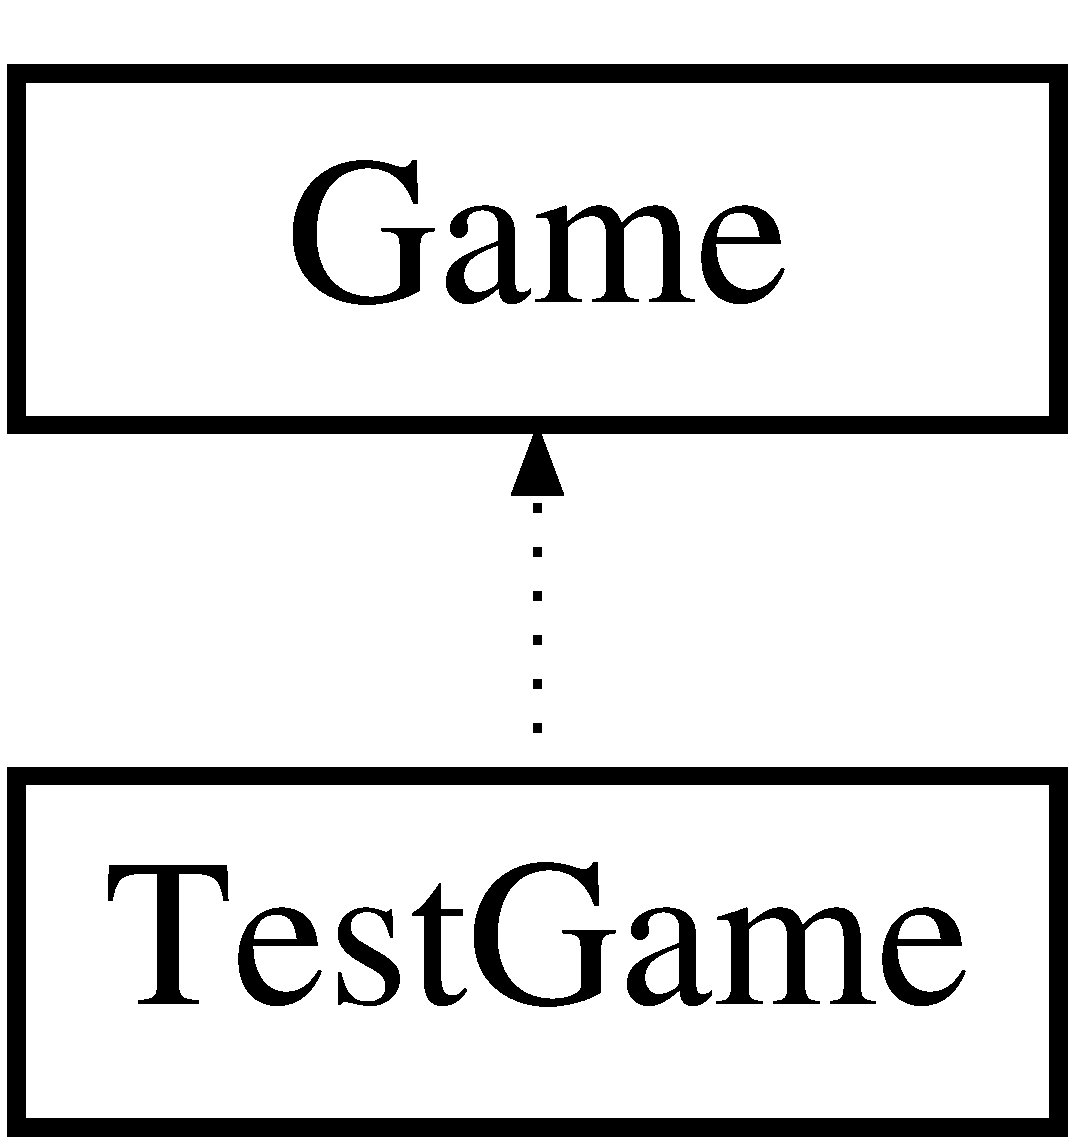
\includegraphics[height=2.000000cm]{class_test_game}
\end{center}
\end{figure}
\subsection*{Additional Inherited Members}


The documentation for this class was generated from the following file\-:\begin{DoxyCompactItemize}
\item 
Test\-Game.\-cpp\end{DoxyCompactItemize}

\addcontentsline{toc}{part}{Index}
\printindex
\end{document}
